\documentclass[12pt,a4paper]{article}

% ─── Page Layout ───────────────────────────────────────────────────────────────
\usepackage[a4paper, margin=0.8in, headheight=14pt]{geometry}

% ─── Fonts (XeLaTeX) ───────────────────────────────────────────────────────────
\usepackage{fontspec}
\usepackage{unicode-math}
\setmainfont{TeX Gyre Pagella}
\setmonofont[Scale=0.88]{TeX Gyre Cursor}
\setmathfont{Latin Modern Math}

% ─── Packages ──────────────────────────────────────────────────────────────────
\usepackage{xcolor}
\usepackage{colortbl}
\usepackage{titlesec}
\usepackage{enumitem}
\usepackage{tabularx}
\usepackage{booktabs}
\usepackage{array}
\usepackage{amsmath}
\usepackage{tikz}
\usetikzlibrary{shapes.geometric, arrows.meta, positioning, calc, fit, decorations.pathreplacing}
\usepackage{tcolorbox}
\tcbuselibrary{skins, breakable}
\usepackage{hyperref}
\usepackage{fancyhdr}
\usepackage{graphicx}
\usepackage{microtype}
\hyphenpenalty=10000
\exhyphenpenalty=10000
\sloppy
\usepackage{caption}
\usepackage{setspace}
\usepackage{multirow}
\usepackage{tocloft}

% ─── Q&A helper ────────────────────────────────────────────────────────────────
\newcommand{\Q}[1]{\textbf{#1}\par\noindent\ignorespaces}

% ─── Colour Palette ────────────────────────────────────────────────────────────
\definecolor{myred}{RGB}{196,30,58}
\definecolor{mydark}{RGB}{30,30,50}
\definecolor{mygreen}{RGB}{14,120,80}
\definecolor{myteal}{RGB}{0,130,140}
\definecolor{myamber}{RGB}{180,100,0}
\definecolor{mypurple}{RGB}{100,30,160}
\definecolor{mygray}{RGB}{246,247,249}
\definecolor{mgframe}{RGB}{180,185,200}
\definecolor{watermark}{RGB}{145,150,170}
\definecolor{hdrred}{RGB}{250,232,235}
\definecolor{hdrgreen}{RGB}{220,244,233}
\definecolor{hdrteal}{RGB}{220,242,244}
\definecolor{hdramber}{RGB}{253,242,215}
\definecolor{hdrpurple}{RGB}{238,228,255}
\definecolor{hdrgray}{RGB}{238,240,245}
\definecolor{rowalt}{RGB}{250,251,253}

% ─── Section Formatting ────────────────────────────────────────────────────────
\titleformat{\section}
  {\large\bfseries\color{myred}}{\thesection.}{0.5em}{}
  [\vspace{1pt}{\color{myred}\rule{\linewidth}{0.8pt}}]
\titleformat{\subsection}
  {\normalsize\bfseries\color{myteal}}{\thesubsection}{0.5em}{}
\titlespacing*{\section}{0pt}{18pt}{7pt}
\titlespacing*{\subsection}{0pt}{11pt}{4pt}

% ─── Paragraph ─────────────────────────────────────────────────────────────────
\setlength{\parindent}{0pt}
\setlength{\parskip}{4pt}

% ─── TOC Styling ───────────────────────────────────────────────────────────────
\renewcommand{\cfttoctitlefont}{\large\bfseries\color{myred}}
\renewcommand{\cftaftertoctitle}{\par\noindent{\color{myred}\rule{\linewidth}{0.8pt}}}
\setlength{\cftbeforetoctitleskip}{0pt}
\setlength{\cftaftertoctitleskip}{6pt}
\renewcommand{\cftsecfont}{\normalsize\bfseries\color{mydark}}
\renewcommand{\cftsecpagefont}{\normalsize\bfseries\color{mydark}}
\renewcommand{\cftsecleader}{\cftdotfill{\cftdotsep}}
\setlength{\cftbeforesecskip}{7pt}
\renewcommand{\cftsubsecfont}{\small\color{mydark}}
\renewcommand{\cftsubsecpagefont}{\small\color{mydark}}
\setlength{\cftbeforesubsecskip}{3pt}
\setlength{\cftsubsecindent}{1.4em}

% ─── Table helpers ─────────────────────────────────────────────────────────────
\renewcommand{\arraystretch}{1.45}
\setlength{\tabcolsep}{6pt}
\arrayrulecolor{mydark}
\newcolumntype{B}[1]{>{\small\bfseries\raggedright\arraybackslash}m{#1}}
\newcolumntype{Y}{>{\small\raggedright\arraybackslash}X}
\renewcommand{\tabularxcolumn}[1]{m{#1}}

% ─── Header / Footer ───────────────────────────────────────────────────────────
\pagestyle{fancy}
\fancyhf{}
\fancyhead[L]{\small\color{myred}\textbf{EC502}\;\color{mydark}--- Computer Architecture}
\fancyhead[R]{\small\color{myteal}\textbf{Module 7 Notes}}
\fancyfoot[C]{\small\color{mydark}\thepage}
\fancyfoot[R]{\small\color{watermark}\textit{\copyright\ Biraj}}
\renewcommand{\headrulewidth}{0.5pt}
\renewcommand{\footrulewidth}{0.3pt}

% ─── Hyperref ──────────────────────────────────────────────────────────────────
\hypersetup{
  colorlinks=true, linkcolor=myteal, urlcolor=myteal,
  pdfauthor={Biraj Sarkar},
  pdftitle={EC502 --- Module 7 Notes}
}

% ─── tcolorbox styles ──────────────────────────────────────────────────────────
\tcbset{
  tikzbox/.style={
    colback=mygray, colframe=mgframe, boxrule=0.6pt, arc=4pt,
    left=8pt, right=8pt, top=6pt, bottom=6pt,
    colbacktitle=mgframe, coltitle=mydark,
    fonttitle=\small\bfseries
  },
  defbox/.style={
    colback=hdrgreen, colframe=mygreen, boxrule=0.8pt, arc=4pt,
    left=9pt, right=9pt, top=6pt, bottom=6pt,
    colbacktitle=mygreen, coltitle=white,
    fonttitle=\small\bfseries
  },
  formulabox/.style={
    colback=hdrteal, colframe=myteal, boxrule=0.8pt, arc=4pt,
    left=9pt, right=9pt, top=7pt, bottom=7pt,
    colbacktitle=myteal, coltitle=white,
    fonttitle=\small\bfseries
  },
  examplebox/.style={
    colback=hdramber, colframe=myamber, boxrule=0.8pt, arc=4pt,
    left=9pt, right=9pt, top=6pt, bottom=6pt,
    colbacktitle=myamber, coltitle=white,
    fonttitle=\small\bfseries
  },
  masonbox/.style={
    colback=hdrpurple, colframe=mypurple, boxrule=0.8pt, arc=4pt,
    left=9pt, right=9pt, top=6pt, bottom=6pt,
    colbacktitle=mypurple, coltitle=white,
    fonttitle=\small\bfseries
  },
  exambox/.style={
    colback=hdrpurple, colframe=mypurple, boxrule=1pt, arc=5pt,
    left=10pt, right=10pt, top=8pt, bottom=8pt,
    colbacktitle=mypurple, coltitle=white,
    fonttitle=\bfseries,
    breakable, title after break={\textbf{Frequently Asked / Viva Questions (contd.)}}}
}
% Make all boxes breakable across pages
\tcbset{breakable}

% ─── TikZ styles ───────────────────────────────────────────────────────────────
\tikzset{
  block/.style={rectangle, draw=myteal, fill=hdrteal,
    text width=2.4cm, align=center, minimum height=0.95cm,
    font=\small, rounded corners=3pt, line width=0.7pt},
  redblock/.style={rectangle, draw=myred, fill=hdrred,
    text width=2.4cm, align=center, minimum height=0.95cm,
    font=\small, rounded corners=3pt, line width=0.7pt},
  netnode/.style={rectangle, draw=myteal, fill=hdrteal,
    text width=1.5cm, align=center, minimum height=0.8cm,
    font=\small, rounded corners=3pt, line width=0.7pt},
  sumjunc/.style={circle, draw=myamber, fill=hdramber,
    minimum size=0.62cm, font=\small, line width=0.8pt},
  snode/.style={circle, draw=mypurple, fill=hdrpurple,
    minimum size=0.55cm, font=\footnotesize, line width=0.7pt},
  arrow/.style={-Stealth, thick, color=mydark},
  redarrow/.style={-Stealth, thick, color=myred},
  line/.style={thick, color=mydark}
}

% ═══════════════════════════════════════════════════════════════════════════════
\begin{document}
% ═══════════════════════════════════════════════════════════════════════════════

\begin{center}
  {\LARGE\bfseries\color{myred} EC502 --- Computer Architecture}\\[5pt]
  {\normalsize\color{mydark} Semester V \quad$\bullet$\quad 3L:0T:0P \quad$\bullet$\quad 3 Credits}\\[3pt]
  {\normalsize\color{myteal}\textbf{Module 7 Exam Notes: Pipelining and Parallel Processing}}\\[3pt]
  {\small\color{mydark} CGEC \;$|$\; B.Tech ECE (2023--27) \;$|$\; \textit{Biraj Sarkar}}
\end{center}
\vspace{2pt}
\noindent{\color{myred}\rule{\linewidth}{1.5pt}}
\vspace{2pt}

\hypersetup{linkcolor=mydark}
\tableofcontents
\hypersetup{linkcolor=myteal}
\newpage

\section{Pipelining and Parallel Processing}
\begin{tcolorbox}[defbox,title={Parallelism and pipeline}]
Parallel processing uses overlapping or simultaneous operations to improve throughput or reduce time for a task. A pipeline splits work into stages and overlaps different items in different stages. Each item still traverses all stages it needs.
\end{tcolorbox}
\subsection{Pipeline stages, clock and speedup}
\begin{tcolorbox}[tikzbox,title={Classic five-stage instruction pipeline},unbreakable]
\centering
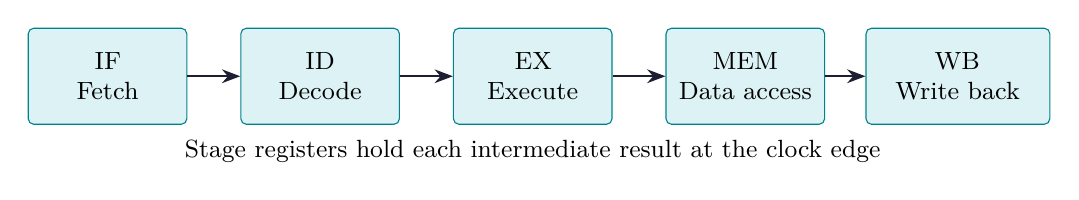
\begin{tikzpicture}[font=\small,stage/.style={draw=myteal,fill=hdrteal,rounded corners=2pt,text width=1.78cm,align=center,minimum height=1.22cm}]
\node[stage] (f) at (0,0) {IF\\Fetch};
\node[stage] (d) at (2.7,0) {ID\\Decode};
\node[stage] (e) at (5.4,0) {EX\\Execute};
\node[stage] (m) at (8.1,0) {MEM\\Data access};
\node[stage,text width=2.10cm] (w) at (10.8,0) {WB\\Write back};
\draw[arrow] (f.east)--(d.west);
\draw[arrow] (d.east)--(e.west);
\draw[arrow] (e.east)--(m.west);
\draw[arrow] (m.east)--(w.west);
\node[below] at (5.4,-.69) {Stage registers hold each intermediate result at the clock edge};
\end{tikzpicture}
\end{tcolorbox}

In a typical load/store design, IF reads the instruction, ID decodes and reads registers, EX calculates an ALU result or address, MEM accesses data for loads and stores, and WB writes a register when required. An arithmetic pipeline applies the same overlap to data operations, such as exponent comparison, alignment, significand addition, normalisation and rounding.
\begin{itemize}[leftmargin=*,itemsep=3pt]
\item \textbf{Clock period.} For logic delays $t_1,\ldots,t_k$ and stage-register overhead $t_r$, take $T_{\rm pipe}=\max_i t_i+t_r$. The longest stage sets the clock.
\item \textbf{Latency and throughput.} With $k$ cycles per item, one item takes $kT_{\rm pipe}$. For an ideal single-issue pipeline the steady completion rate is one item per cycle. Including fill and drain, $n$ items take $(k+n-1)T_{\rm pipe}$.
\item \textbf{Speedup.} If the nonpipelined reference runs each item in $\sum_i t_i$ without register overhead, speedup is $n\sum_i t_i/[(k+n-1)T_{\rm pipe}]$. For equal stage lengths and no overhead this becomes $kn/(k+n-1)$, approaching $k$ for large $n$.
\item \textbf{Efficiency.} Under the equal-stage ideal model, speedup divided by $k$ is $n/(k+n-1)$, the average fraction of occupied stage slots over the run. Count stalls separately if present.
\end{itemize}
\begin{tcolorbox}[examplebox,title={Unequal stages and finite workload}]
Four stage delays are $10,15,12,8\,\mathrm{ns}$ and each pipeline register adds $2\,\mathrm{ns}$. The pipeline clock is $17\,\mathrm{ns}$. For 20 items, nonpipelined time is $20(45)=900\,\mathrm{ns}$ and pipelined time is $(4+20-1)17=391\,\mathrm{ns}$, speedup $2.30$. One pipeline item takes $68\,\mathrm{ns}$ whereas one nonpipelined item takes $45\,\mathrm{ns}$. Overlap improves throughput even when single-item latency increases.
\end{tcolorbox}

\section{Pipeline Dependencies, Hazards and Control}
\begin{tcolorbox}[defbox,title={Pipeline hazard}]
A hazard is a condition that prevents an instruction from safely proceeding in its scheduled cycle. Resolve it by scheduling around it, forwarding an available value, stalling, or recovering from a wrong prediction.
\end{tcolorbox}
\par\vspace{6pt}\noindent
\begin{tabularx}{\linewidth}{|B{2.55cm}|Y|Y|}\hline
Hazard & Cause and example & Standard remedy \\ \hline
Structural & Two stages need the same resource in a cycle, such as instruction fetch and a load on one single-ported memory. & Arbitrate and stall, or use separate ports or instruction/data paths. \\ \hline
Data & An instruction reads a register before an earlier instruction's result is available (read after write, RAW). & Forward from a later stage when ready. Stall when the producer is still too late. \\ \hline
Control & The next PC depends on an unresolved branch or jump. & Wait, resolve early, or predict and flush wrong-path instructions on a miss. \\ \hline
\end{tabularx}

\subsection{RAW, WAR and WAW}
\begin{itemize}[leftmargin=*,itemsep=3pt]
\item \textbf{RAW, true dependence.} A consumer needs the value produced by an earlier instruction. A forwarding mux can route it from an execution or memory stage instead of waiting for register write-back.
\item \textbf{WAR, anti-dependence.} A younger write must wait until an older instruction has read the old value. \textbf{WAW, output dependence:} an older write must not replace a newer write to the same architectural register.
\item \textbf{When WAR and WAW matter.} Fixed in-order reads in ID and in-order writes in WB of a classic pipeline preserve order. Variable-latency or out-of-order execution may need register renaming to remove artificial name dependencies and ordered retirement to expose correct results.
\end{itemize}
\begin{tcolorbox}[examplebox,title={Load-use hazard with forwarding}]
Assume load data is ready at the end of MEM and ALU inputs are needed at the start of EX. The load's immediate consumer must stall one cycle. EX of SUB can receive ADD's ALU result by forwarding. A repeated stage label with an asterisk is a held or retried stage.
\par\vspace{6pt}\noindent
\begin{tabularx}{\linewidth}{|B{3.0cm}|*{8}{>{\centering\arraybackslash\small}X|}}\hline
Instruction & 1 & 2 & 3 & 4 & 5 & 6 & 7 & 8 \\ \hline
\texttt{LD R1,[R2]} & IF & ID & EX & MEM & WB & & & \\ \hline
\texttt{ADD R3,R1,R4} & & IF & ID & ID$^*$ & EX & MEM & WB & \\ \hline
\texttt{SUB R5,R3,R6} & & & IF & IF$^*$ & ID & EX & MEM & WB \\ \hline
\end{tabularx}

The hazard unit freezes the PC and the fetch/decode register for one cycle and inserts a bubble into EX in cycle 4. The load advances to MEM and its data forwards to ADD in cycle 5.
\end{tcolorbox}

\subsection{Branch control and effective CPI}
For a resolved or correctly predicted next PC, fetching can continue. On misprediction, redirect fetch and flush the younger wrong-path instructions before they change architectural state. The branch penalty depends on the resolution stage and fetch logic.
\begin{tcolorbox}[examplebox,title={Sum independent stall contributions}]
Assume base CPI 1. If $25\%$ of instructions are loads and $20\%$ of those loads have an immediate use costing one stall, the load contribution is $0.25(0.20)(1)=0.05$. If $18\%$ of instructions are branches, $10\%$ of branches are mispredicted and each costs 3 cycles, the branch contribution is $0.18(0.10)(3)=0.054$. Ignoring overlap and other stalls, effective CPI is $1.104$. Multiply this by instruction count and clock period to find CPU time.
\end{tcolorbox}

\section{Forms of Parallel Processing}
\subsection{Flynn's classification}
Classify by how many instruction and data streams are active. Streams describe logical execution, not the number of pipeline stages.
\par\vspace{6pt}\noindent
\begin{tabularx}{\linewidth}{|B{2.3cm}|Y|Y|}\hline
Class & Streams & Representative organisation \\ \hline
SISD & Single instruction, single data & Conventional single instruction stream over one data stream. It can still use a pipeline internally. \\ \hline
SIMD & Single instruction, multiple data & One operation controls several data lanes. Vector instructions and array processors are common examples. \\ \hline
MISD & Multiple instruction, single data & Different processing operations on the same logical data stream. Uncommon as a general-purpose organisation. \\ \hline
MIMD & Multiple instruction, multiple data & Independent instruction streams on separate cores or nodes. \\ \hline
\end{tabularx}

\begin{itemize}[leftmargin=*,itemsep=4pt]
\item \textbf{Instruction-level parallelism.} Pipelining overlaps instructions. A superscalar CPU can start more than one independent instruction per cycle. Dependencies and available issue units limit useful overlap.
\item \textbf{Very long instruction word (VLIW).} The compiler schedules independent operations into explicit bundles for several units. This can simplify issue hardware. Code scheduled for a particular bundle format or timing model may need recompilation for another implementation.
\item \textbf{Data-level parallelism.} A vector processor applies vector instructions to elements through vector lanes or pipelines. An array processor uses a collection of processing elements controlled together. Both exploit repeated operations over elements.
\item \textbf{Task or thread parallelism.} Separate tasks or threads run on multiple cores. A shared-memory multiprocessor gives processors a common address space. A distributed-memory multicomputer uses private memory per node and exchanges messages.
\item \textbf{Shared memory variants.} Uniform memory access (UMA) abstracts similar memory access cost across processors. Non-uniform memory access (NUMA) has different local and remote costs. Both may still expose one address space.
\end{itemize}
\subsection{Synchronization, coherence and speedup limits}
\begin{itemize}[leftmargin=*,itemsep=3pt]
\item \textbf{Race.} Two cores reading the same counter and independently writing back incremented values can lose an update. Protect the critical section with a lock built on atomic operations, or use atomic increment where suitable.
\item \textbf{Barrier.} Workers finish their current phase before any proceeds to the next. In a message-passing system, explicit sends and receives communicate data and coordinate dependencies.
\item \textbf{Coherence and ordering.} Coherence governs observations of writes to a single address across caches. Memory consistency specifies allowed orderings across accesses, including different addresses. Use the synchronization primitives defined by the programming model.
\item \textbf{Speedup limit.} If a serial fraction $f_s$ remains, ideal speedup on $p$ workers is $1/[f_s+(1-f_s)/p]$. With $f_s=0.10$ and eight workers, it is $4.71$, even before communication, imbalance and synchronization costs.
\end{itemize}
\begin{tcolorbox}[examplebox,title={Follow a coherence invalidation}]
Both cores cache a line holding $X=0$. When core A requests write ownership to store 1, an invalidation protocol invalidates core B's shared copy before granting exclusive write permission. After a properly synchronised handoff, core B's next load can obtain the updated value from the owner or coherent memory system. A shared writable region can instead be mapped uncached on a suitable system, using the platform's ordering rules, at the cost of extra memory traffic. A lock or barrier also supplies ordering, but does not by itself repair stale cache data on a non-coherent system.
\end{tcolorbox}

% Keep the heading and definition together where the preceding box ends low on a page.
\par
\ifdim\dimexpr\pagegoal-\pagetotal\relax<108pt\relax
  \newpage
\fi
\section{Interconnection Networks}
\begin{tcolorbox}[defbox,title={Interconnect}]
An interconnection network carries requests and responses among processors, memories and I/O endpoints. Topology says which links exist. Routing chooses a path, and flow control manages use of links and buffers.
\end{tcolorbox}
\par\vspace{6pt}\noindent
\begin{tabularx}{\linewidth}{|B{2.8cm}|Y|Y|}\hline
Topology & Paths & Main cost or limitation \\ \hline
Bus & One shared communication medium. & Low wiring cost. Arbitration and shared bandwidth limit scaling. \\ \hline
Ring & Nodes connect to neighbours in a loop. & Small node degree. Messages may traverse several hops. \\ \hline
Mesh & Nodes connect to nearby grid neighbours. & Regular wiring. Distant communication takes multiple hops. \\ \hline
Crossbar & Crosspoints connect each input to each output. & Nonblocking for connections to distinct outputs. An $N$ by $N$ crossbar needs $N^2$ crosspoints. \\ \hline
Omega network & $\log_2 N$ stages of $2$ by $2$ switches with shuffle links for $N=2^k$. & Uses $(N/2)\log_2N$ switches, but internal conflicts can block distinct-output routes. \\ \hline
\end{tabularx}

\begin{tcolorbox}[tikzbox,title={Crossbar example: concurrent requests to different outputs},unbreakable]
\centering
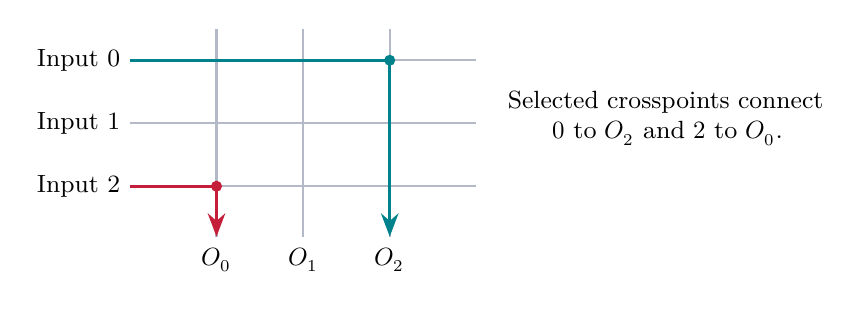
\begin{tikzpicture}[font=\small,x=1.1cm,y=.8cm]
\foreach \i in {0,1,2}{
 \draw[mgframe,thick] (0,2-\i)--(4,2-\i);
 \node[left] at (0,2-\i) {Input \i};
 \draw[mgframe,thick] (1+\i,2.5)--(1+\i,-.8);
 \node[below] at (1+\i,-.82) {$O_{\i}$};
}
\draw[myteal,very thick,-Stealth] (0,2)--(3,2)--(3,-.8);
\draw[myred,very thick,-Stealth] (0,0)--(1,0)--(1,-.8);
\fill[myteal] (3,2) circle (2pt);
\fill[myred] (1,0) circle (2pt);
\node[align=center,text width=4cm,anchor=west] at (4.25,1.08) {Selected crosspoints connect $0$ to $O_2$ and $2$ to $O_0$.};
\end{tikzpicture}
\end{tcolorbox}
\subsection{A multistage routing example}
In an eight-input Omega convention in which adjacent inputs share the first switch, successive destination bits choose the upper or lower output link at each stage, most significant first. The interstage shuffle permutes link positions. There are $3$ stages of $4$ switches, or 12 switches total. Input 0 to destination \texttt{000} and input 1 to destination \texttt{001} need the same upper output of their first switch because both destination high bits are 0. They can contend even though their final outputs differ. In a crossbar the two distinct outputs could be selected concurrently. Evaluate networks by switch/wire cost, latency, bandwidth, blocking and scalability.

\newpage
\begin{center}
  {\large\bfseries\color{myred} Quick Revision --- Module 7}\\[3pt]
  {\small\color{mydark} Pipelining and Parallel Processing $|$ EC502}
\end{center}
\noindent{\color{myred}\rule{\linewidth}{1.2pt}}
\begin{tcolorbox}[formulabox,title={Key Formulas at a Glance}]
\renewcommand{\arraystretch}{1.35}
\begin{tabularx}{\linewidth}{B{5.0cm}Y}
Ideal pipeline time & $(k+n-1)T_{\rm pipe}$ for $n$ items and $k$ stages \\[3pt]
Pipeline period & $\max_i(t_i)+t_r$ \\[3pt]
Effective CPI & Base CPI plus weighted stall cycles per instruction \\[3pt]
Parallel speedup & $1/[f_s+(1-f_s)/p]$ under ideal workload split \\[3pt]
Omega switch count & $(N/2)\log_2 N$ for a power-of-two port count \\[3pt]
\end{tabularx}
\end{tcolorbox}
\begin{tcolorbox}[defbox,title={One-Line Definitions}]
\textbf{Forwarding.} Route a ready result directly to a later consumer stage.\par
\textbf{Bubble.} Empty or invalid pipeline slot that makes no architectural update.\par
\textbf{Array processor.} Multiple processing elements operated together on different data.\par
\end{tcolorbox}
\begin{tcolorbox}[exambox,title={Frequently Asked / Viva Questions}]
\begin{enumerate}[topsep=0pt, label=\textbf{Q\arabic*.}, itemsep=5pt]
\item \Q{Does a pipeline necessarily reduce one instruction's latency?}
No. Its main benefit is overlapping work to raise throughput.
\item \Q{What sets the pipeline clock period?}
The slowest stage plus register overhead.
\item \Q{When does load-use still stall with forwarding?}
When load data becomes available after the dependent instruction needs it.
\item \Q{What is a structural hazard?}
Multiple operations request an insufficiently replicated resource at the same time.
\item \Q{Are WAR and WAW true value dependencies?}
No. They arise from reuse of a destination name.
\item \Q{What happens on a branch misprediction?}
Wrong-path work is flushed and fetch restarts at the correct PC.
\item \Q{How do vector and array processors exploit data parallelism?}
Vector instructions operate on sequences using lanes or pipelines. Array processors use multiple controlled processing elements.
\item \Q{What defines MIMD?}
Multiple instruction streams operating on multiple data streams.
\item \Q{Why use a barrier?}
No worker in the next phase proceeds until participating workers finish the current phase.
\item \Q{Why can a multistage network block two distinct destinations?}
Both paths may require the same internal link.
\end{enumerate}
\end{tcolorbox}
\begin{tcolorbox}[tikzbox,title={Summary comparison}]
\begin{tabularx}{\linewidth}{|B{4cm}|Y|}\hline
\textbf{Case} & \textbf{What to use} \\ \hline
Pipelining & Overlap stages of different work items. \\ \hline
SIMD / MIMD & Shared operation on several data items / independent instruction streams. \\ \hline
Crossbar / Omega & More crosspoints with flexible distinct-output paths / fewer switches with possible internal contention. \\ \hline
\end{tabularx}
\end{tcolorbox}
\end{document}
